% LEGACY/NON-SUBMISSION ARTIFACT.
% The active manuscript for the repaired evidence path is
% paper/conference_draft.tex. This older journal draft retains stale
% stored-recommendation-table claims (for example 19 recommendations and
% about $590/month) for provenance only and should not be submitted.
\documentclass[10pt,journal]{IEEEtran}
\IEEEoverridecommandlockouts

\usepackage{cite}
\usepackage{amsmath,amssymb,amsfonts}
\usepackage{amsthm}
\usepackage{algorithm}
\usepackage{algpseudocode}
\usepackage{graphicx}
\usepackage{booktabs}
\usepackage{array}
\usepackage{multirow}
\usepackage{xcolor}
\usepackage{url}
\usepackage[hidelinks]{hyperref}
\usepackage{microtype}

% --- numbers generated from the database and the public traces -------------
% make_figures.py          -> numbers.tex          (synthetic account study)
% external_validation.py   -> numbers_external.tex (Bitbrains/Materna traces)
% policy_sim.py            -> numbers_policy.tex   (policy sim, synthetic)
% policy_sim.py --csv ...  -> numbers_policy_ext.tex (policy sim, real trace)
% Auto-generated by paper/make_figures.py -- do not edit by hand.
\newcommand{\totalBill}{2189.48}
\newcommand{\totalSavings}{590.40}
\newcommand{\savingsPctBill}{27.0}
\newcommand{\savingsPctBillExact}{26.97}
\newcommand{\savingsPctFlagged}{54.9}
\newcommand{\flaggedCost}{1074.83}
\newcommand{\afterCost}{484.43}
\newcommand{\numRecs}{19}
\newcommand{\numAiRecs}{10}
\newcommand{\numEctwo}{8}
\newcommand{\numResources}{42}
\newcommand{\numServicesBilled}{6}
\newcommand{\nDays}{365}
\newcommand{\dataStart}{2024-07-01}
\newcommand{\dataEnd}{2025-06-30}
\newcommand{\meanDaily}{74.64}
\newcommand{\stdDaily}{22.87}
\newcommand{\minDaily}{36.10}
\newcommand{\maxDaily}{232.52}
\newcommand{\annualTotal}{27,243.31}
\newcommand{\surgeThresh}{120.38}
\newcommand{\numSurges}{5}
\newcommand{\maxZ}{6.9}
\newcommand{\savRightsize}{362.81}
\newcommand{\cntRightsize}{2}
\newcommand{\savPricing}{208.42}
\newcommand{\cntPricing}{6}
\newcommand{\savDelete}{10.00}
\newcommand{\cntDelete}{3}
\newcommand{\savNat}{5.67}
\newcommand{\cntNat}{2}
\newcommand{\savEbs}{2.60}
\newcommand{\cntEbs}{4}
\newcommand{\savSthree}{0.79}
\newcommand{\cntSthree}{1}
\newcommand{\savLambda}{0.11}
\newcommand{\cntLambda}{1}
\newcommand{\savHigh}{370.52}
\newcommand{\cntHigh}{8}
\newcommand{\savMed}{214.21}
\newcommand{\cntMed}{9}
\newcommand{\savLow}{5.67}
\newcommand{\cntLow}{2}
\newcommand{\mapeSnaive}{12.3}
\newcommand{\mapeEts}{11.2}
\newcommand{\mapeProphet}{20.9}
\newcommand{\mapeNaive}{27.3}
\newcommand{\bestModel}{ETS}
\newcommand{\bestMape}{11.2}
\newcommand{\holdoutModel}{ETS}
\newcommand{\holdoutMape}{12.0}
\newcommand{\holdoutCov}{97}
\newcommand{\cvInitial}{120}
\newcommand{\cvStep}{30}

% Auto-generated by paper/external_validation.py -- do not edit by hand.
\newcommand{\extSnapshot}{2026-06-30}
\newcommand{\extCatalogSize}{28}
\newcommand{\extFsVms}{1250}
\newcommand{\extFsBaseline}{128,588}
\newcommand{\extFsOptimized}{85,414}
\newcommand{\extFsSavingsPct}{33.6}
\newcommand{\extFsSavingsPctRi}{58.3}
\newcommand{\extFsDownsized}{765}
\newcommand{\extFsUpsized}{181}
\newcommand{\extFsClamped}{0}
\newcommand{\extRndVms}{500}
\newcommand{\extRndBaseline}{44,294}
\newcommand{\extRndOptimized}{29,614}
\newcommand{\extRndSavingsPct}{33.1}
\newcommand{\extRndSavingsPctRi}{58.0}
\newcommand{\extRndDownsized}{301}
\newcommand{\extRndUpsized}{57}
\newcommand{\extRndClamped}{0}
\newcommand{\extMatVms}{547}
\newcommand{\extMatBaseline}{44,184}
\newcommand{\extMatOptimized}{11,398}
\newcommand{\extMatSavingsPct}{74.2}
\newcommand{\extMatSavingsPctRi}{83.8}
\newcommand{\extMatDownsized}{509}
\newcommand{\extMatUpsized}{4}
\newcommand{\extMatClamped}{0}
\newcommand{\extGammaReal}{0.63}
\newcommand{\extTotalVms}{2,297}
\newcommand{\extRndHours}{2142}
\newcommand{\extRndMeanGhz}{402.4}
\newcommand{\extRndSurges}{149}
\newcommand{\extMapeNaive}{82.3}
\newcommand{\extMapeSdNaive}{66.6}
\newcommand{\extMaseNaive}{0.91}
\newcommand{\extCovNaive}{95}
\newcommand{\extMapeSnaive}{65.0}
\newcommand{\extMapeSdSnaive}{40.3}
\newcommand{\extMaseSnaive}{1.35}
\newcommand{\extCovSnaive}{74}
\newcommand{\extMapeEts}{77.0}
\newcommand{\extMapeSdEts}{57.2}
\newcommand{\extMaseEts}{0.93}
\newcommand{\extCovEts}{54}
\newcommand{\extMapeProphet}{60.8}
\newcommand{\extMapeSdProphet}{21.6}
\newcommand{\extMaseProphet}{1.01}
\newcommand{\extCovProphet}{62}
\newcommand{\extBestModel}{Prophet}
\newcommand{\extBestMape}{60.8}
\newcommand{\extNFolds}{9}
\newcommand{\extDmStat}{-1.20}
\newcommand{\extDmP}{0.232}
\newcommand{\extWilcoxonP}{0.570}
\newcommand{\extDmPProphetSnaive}{0.235}
\newcommand{\extDmPProphetNaive}{0.604}
\newcommand{\extAnyBestMape}{48.2}
\newcommand{\extDailyMapeNaive}{53.4}
\newcommand{\extDailyMapeSdNaive}{14.2}
\newcommand{\extDailyMaseNaive}{1.32}
\newcommand{\extDailyMapeSnaive}{54.2}
\newcommand{\extDailyMapeSdSnaive}{22.6}
\newcommand{\extDailyMaseSnaive}{1.26}
\newcommand{\extDailyMapeEts}{52.1}
\newcommand{\extDailyMapeSdEts}{29.9}
\newcommand{\extDailyMaseEts}{1.10}
\newcommand{\extDailyMapeProphet}{59.8}
\newcommand{\extDailyMapeSdProphet}{36.9}
\newcommand{\extDailyMaseProphet}{1.26}
\newcommand{\extDailyBestModel}{ETS}
\newcommand{\extDailyBestMape}{52.1}
\newcommand{\extDailyNFolds}{7}
% Additional Study II reproducibility macros from paper/study2_reproducibility.py.
\newcommand{\extFsSavingsCiLow}{24.5}
\newcommand{\extFsSavingsCiHigh}{41.8}
\newcommand{\extFsSavingsPctRiCiLow}{52.5}
\newcommand{\extFsSavingsPctRiCiHigh}{63.5}
\newcommand{\extRndSavingsCiLow}{19.3}
\newcommand{\extRndSavingsCiHigh}{46.3}
\newcommand{\extRndSavingsPctRiCiLow}{49.3}
\newcommand{\extRndSavingsPctRiCiHigh}{66.3}
\newcommand{\extMatSavingsCiLow}{71.4}
\newcommand{\extMatSavingsCiHigh}{76.8}
\newcommand{\extMatSavingsPctRiCiLow}{82.1}
\newcommand{\extMatSavingsPctRiCiHigh}{85.4}
\newcommand{\extOverallSavingsPct}{41.8}
\newcommand{\extOverallSavingsCiLow}{35.9}
\newcommand{\extOverallSavingsCiHigh}{47.5}
\newcommand{\extOverallSavingsPctRi}{63.4}
\newcommand{\extOverallSavingsPctRiCiLow}{59.7}
\newcommand{\extOverallSavingsPctRiCiHigh}{67.0}

% Auto-generated by paper/azure_validation.py -- do not edit by hand.
\newcommand{\azVms}{237,272}
\newcommand{\azTotalRows}{2,695,548}
\newcommand{\azDroppedBucket}{10,923}
\newcommand{\azDroppedShort}{2,447,247}
\newcommand{\azBaseline}{16,670,839}
\newcommand{\azOptimized}{17,307,607}
\newcommand{\azSavingsPct}{-3.8}
\newcommand{\azSavingsPctRi}{34.8}
\newcommand{\azDownsized}{21,772}
\newcommand{\azUpsized}{26,227}

% Auto-generated by paper/policy_sim.py -- do not edit by hand.
\newcommand{\polGammaStar}{0.63}
\newcommand{\polTrainPeriods}{219}
\newcommand{\polTestPeriods}{146}
% Deprecated *Days aliases retained for finalized conference/main consumers; values count periods (sampling period: day). Use *Periods in new prose.
\newcommand{\polTrainDays}{219}
\newcommand{\polTestDays}{146}
\newcommand{\polPctHeur}{101.8}
\newcommand{\polPctNv}{73.6}
\newcommand{\polPctSaa}{73.6}
\newcommand{\polPctLookSeven}{74.1}
\newcommand{\polPctLookThirty}{73.3}
\newcommand{\polPctLookSixty}{73.4}
\newcommand{\polPctDual}{72.8}
\newcommand{\polPctDualc}{74.6}
\newcommand{\polPctLb}{63.0}
\newcommand{\polPoC}{28.2}
\newcommand{\polImpliedQ}{99}
\newcommand{\polSurgeTrain}{3}
\newcommand{\polSurgeTest}{2}
\newcommand{\polNvSave}{26.4}
\newcommand{\polDualGain}{0.8}
\newcommand{\polDualcGain}{-1.0}
\newcommand{\polDualGapCapture}{7}
\newcommand{\polDualcGapCapture}{-10}
\newcommand{\polHeurBreakeven}{0.62}
\newcommand{\polDualGainThreshMin}{-0.6}
\newcommand{\polDualGainThreshMax}{0.8}
\newcommand{\polDualcGainThreshMin}{-3.0}
\newcommand{\polDualcGainThreshMax}{-1.0}
\newcommand{\polDualcGainHoldOne}{-1.0}
\newcommand{\polNvSaveMin}{26.1}
\newcommand{\polNvSaveMax}{26.4}
\newcommand{\polPoCMin}{22.6}
\newcommand{\polPoCMax}{28.2}
% Empirical commitment-proxy Q values; units are arm-specific.
\newcommand{\polQheur}{125.3}
\newcommand{\polQnv}{68.8}
\newcommand{\polQlookSeven}{82.0}
\newcommand{\polQlookThirty}{73.1}
\newcommand{\polQlookSixty}{72.7}
\newcommand{\polLookSevenPeriods}{7}
\newcommand{\polLookThirtyPeriods}{30}
\newcommand{\polLookSixtyPeriods}{60}
\newcommand{\polQdualbase}{68.5}
\newcommand{\polQdualsurge}{195.7}
% Deprecated K-named aliases for finalized conference/main consumers.
\newcommand{\polKheur}{\polQheur}
\newcommand{\polKnv}{\polQnv}
\newcommand{\polKlookSeven}{\polQlookSeven}
\newcommand{\polKlookThirty}{\polQlookThirty}
\newcommand{\polKlookSixty}{\polQlookSixty}
\newcommand{\polKdualbase}{\polQdualbase}
\newcommand{\polKdualsurge}{\polQdualsurge}
\newcommand{\polSaaNvGapPct}{0.57}
\newcommand{\polOdMonthly}{2,388.62}
\newcommand{\polHeurMonthly}{2,432.01}
\newcommand{\polNvMonthly}{1,757.46}
\newcommand{\polPoCMonthly}{674.55}

% Auto-generated by paper/policy_sim.py -- do not edit by hand.
\newcommand{\extPolGammaStar}{0.63}
\newcommand{\extPolTrainPeriods}{1285}
\newcommand{\extPolTestPeriods}{857}
% Deprecated *Days aliases retained for finalized conference/main consumers; values count periods (sampling period: hour). Use *Periods in new prose.
\newcommand{\extPolTrainDays}{1285}
\newcommand{\extPolTestDays}{857}
\newcommand{\extPolPctHeur}{153.5}
\newcommand{\extPolPctNv}{86.2}
\newcommand{\extPolPctSaa}{86.2}
\newcommand{\extPolPctLookSeven}{91.2}
\newcommand{\extPolPctLookThirty}{84.9}
\newcommand{\extPolPctLookSixty}{86.2}
\newcommand{\extPolPctDual}{77.7}
\newcommand{\extPolPctDualc}{78.1}
\newcommand{\extPolPctLb}{63.0}
\newcommand{\extPolPoC}{67.4}
\newcommand{\extPolImpliedQ}{100}
\newcommand{\extPolSurgeTrain}{54}
\newcommand{\extPolSurgeTest}{124}
\newcommand{\extPolNvSave}{13.8}
\newcommand{\extPolDualGain}{8.5}
\newcommand{\extPolDualcGain}{8.1}
\newcommand{\extPolDualGapCapture}{37}
\newcommand{\extPolDualcGapCapture}{35}
\newcommand{\extPolDualGainThreshMin}{2.8}
\newcommand{\extPolDualGainThreshMax}{8.5}
\newcommand{\extPolDualcGainThreshMin}{2.7}
\newcommand{\extPolDualcGainThreshMax}{8.1}
\newcommand{\extPolDualcGainHoldOne}{8.1}
\newcommand{\extPolNvSaveMin}{12.5}
\newcommand{\extPolNvSaveMax}{16.0}
\newcommand{\extPolPoCMin}{45.8}
\newcommand{\extPolPoCMax}{116.4}
% Empirical commitment-proxy Q values; units are arm-specific.
\newcommand{\extPolQheur}{1096248.9}
\newcommand{\extPolQnv}{203631.6}
\newcommand{\extPolQlookSeven}{511981.0}
\newcommand{\extPolQlookThirty}{268870.3}
\newcommand{\extPolQlookSixty}{203631.6}
\newcommand{\extPolLookSevenPeriods}{168}
\newcommand{\extPolLookThirtyPeriods}{720}
\newcommand{\extPolLookSixtyPeriods}{1285}
\newcommand{\extPolQdualbase}{197302.0}
\newcommand{\extPolQdualsurge}{936657.4}
% Deprecated K-named aliases for finalized conference/main consumers.
\newcommand{\extPolKheur}{\extPolQheur}
\newcommand{\extPolKnv}{\extPolQnv}
\newcommand{\extPolKlookSeven}{\extPolQlookSeven}
\newcommand{\extPolKlookThirty}{\extPolQlookThirty}
\newcommand{\extPolKlookSixty}{\extPolQlookSixty}
\newcommand{\extPolKdualbase}{\extPolQdualbase}
\newcommand{\extPolKdualsurge}{\extPolQdualsurge}
\newcommand{\extPolSaaNvGapPct}{0.12}


\newcommand{\E}{\mathbb{E}}
\newcommand{\R}{\mathbb{R}}
\newcommand{\pos}[1]{\left(#1\right)^{+}}
\graphicspath{{figures/}}

\newtheorem{proposition}{Proposition}
\newtheorem{definition}{Definition}
\newtheorem{remark}{Remark}

\begin{document}

\title{A Data-Driven Capacity-Reservation System for\\
Cloud Cost Optimization under Intermittent Demand Surges}

\author{First~Author,
        Second~Author,
        and~Third~Author%
\thanks{The authors are with the Department of Scientific Computing, Faculty
of Computer and Information Sciences, \textit{Affiliation Placeholder}, City,
Country (e-mail: \{author1, author2, author3\}@example.edu).}%
\thanks{Manuscript received July 2026. \textit{(Author block is a placeholder;
fill before submission.)}}}

\markboth{Preprint --- under review}%
{Author \MakeLowercase{\textit{et al.}}: A Data-Driven Capacity-Reservation System for Cloud Cost Optimization}

\maketitle

\begin{abstract}
Conservative fractile heuristics---sizing capacity at a high percentile of
observed utilization plus headroom---are standard practice in cloud
right-sizing, while operations-management theory prescribes
newsvendor-fractile sizing of reserved capacity under two-tier pricing. What
this conservatism costs when carried over to reservation sizing has been, to
our knowledge, unquantified. We bridge practice and theory. Smart Cloud Optimizer
operationalizes the capacity-reservation policy as a pipeline of
walk-forward-validated forecasting, mixed-integer right-sizing at an
empirical $q_{0.95}{\times}1.3$ fractile, and reservation actions gated on
always-on usage; on a \nDays-day \emph{synthetic} AWS account it emits
\numRecs{} recommendations worth \savingsPctBill\% of the \$\totalBill/month
bill. An out-of-sample policy simulation then prices the heuristic: at the
catalog reserved/on-demand ratio $\gamma{=}\polGammaStar$, the deployed
fractile---read counterfactually as a reservation-sizing rule---would
realize \polPctHeur\% (synthetic) and
\extPolPctHeur\% (real trace) of pure on-demand cost, forfeiting the entire
discount. The newsvendor fractile instead realizes
\polPctNv\%/\extPolPctNv\%, and a two-tier base/supplementary policy
\polPctDual\%/\extPolPctDual\%; a causal variant retains nearly all of that
gain on real demand. On \emph{real} telemetry
(\extTotalVms{} VMs from the Bitbrains and Materna public traces),
mixed-integer right-sizing over a verified AWS catalog saves
\extRndSavingsPct--\extMatSavingsPct\% against a like-for-like
lift-and-shift baseline, rising to
\extRndSavingsPctRi--\extMatSavingsPctRi\% with one-year reservations; on a
\azVms-VM Azure fleet with max-based percentiles and unmeasured memory,
right-sizing alone turns cost-negative while reservations still save
\azSavingsPctRi\%. Point
forecasts never significantly beat seasonal-naive baselines, and
real-aggregate forecast error never falls below \extAnyBestMape\%
MAPE---supporting sizing from demand \emph{quantiles}. Every number is
script-regenerated from raw data to compiled PDF. The deployed always-on
reservation gate avoids the penalty we measure.
\end{abstract}

\begin{IEEEkeywords}
cloud cost optimization, capacity reservation, newsvendor, reserved instances,
time-series forecasting, mixed-integer programming, FinOps.
\end{IEEEkeywords}

\IEEEpeerreviewmaketitle

% =====================================================================
\section{Introduction}\label{sec:intro}
% =====================================================================
\IEEEPARstart{P}{ublic-cloud} adoption continues to accelerate, but cost
governance has not kept pace: industry surveys consistently report that
roughly a quarter to a third of cloud spend is wasted on idle or
over-provisioned resources~\cite{flexera2024soc,everman2022waste}, hyperscaler
telemetry shows chronic over-provisioning at the VM
level~\cite{cortez2017resource,reidys2025coach}, and a recent production trace
of $48{,}000$ enterprise VMs found more than $80\%$ using under $70\%$ of
their provisioned resources~\cite{uhlig2025sap}. The root cause is a mismatch
between how demand behaves and how capacity is priced. Demand for a typical
workload is a \emph{base} load---low, stationary, and
predictable---punctuated by intermittent \emph{surges} driven by promotions,
launches, batch jobs, or seasonal
events~\cite{fox2009berkeley,shen2015bitbrains,tirmazi2020borgng}. Pricing,
meanwhile, is two-sided: a \emph{reserved} (committed) tariff that is cheap
per unit but is paid whether used or not, and an \emph{on-demand} tariff that
is elastic with zero commitment but costs substantially more per unit.
Choosing how much capacity to reserve versus leave to on-demand is therefore
a classic trade-off between commitment risk and elasticity premium.

Chen, Lei, and Moinzadeh~\cite{chen2024capacity} formalize this trade-off as
a capacity-reservation problem. A firm holds \emph{base contracts} sized to
the stationary base demand and \emph{supplementary contracts} for surges;
demand beyond reserved capacity spills to on-demand. They show that the
cost-optimal capacities follow a \emph{newsvendor critical fractile}, and
that the optimal management of supplementary contracts (purchase, renewal,
cancellation, expiration) is a two-threshold $(s,S)$ policy. This is a
closed-form \emph{characterization}, but it presumes the demand distributions
are known and deterministic in structure, and it produces a policy rather
than an operational pipeline that an engineering team can run against a real
account.

A parallel systems literature attacks the same waste
empirically---forecasting utilization and reacting with autoscaling or
instance
acquisition~\cite{chaisiri2012provisioning,wang2014optimal,hosseini2020switch,kirchoff2024provisioning,agullo2025forecasting,rzadca2020autopilot}---but
rarely connects its heuristics back to the cost-optimal reservation policy,
and seldom reports end-to-end dollar savings with a reproducible methodology.
The two bodies of work are complementary: one supplies the economic optimum,
the other supplies the data and tooling.

\textbf{This paper bridges the two.} We present \emph{Smart Cloud Optimizer},
a system that operationalizes the base/supplementary/on-demand reservation
framework of~\cite{chen2024capacity} on account telemetry, and---new relative
to prior operationalizations---we measure, in both directions, what the
bridge is worth: what the theory gains from real data, and what deployed
practice would gain from the theory. Our contributions are:

\begin{enumerate}
\item \textbf{An end-to-end system realizing a reservation policy}
(Section~\ref{sec:system}): a mixed-integer linear program (MILP) sizes
capacity at a fixed empirical fractile (the $95$th percentile of observed
utilization with $1.3\times$ headroom---the same percentile idiom used by
production limit-setters such as Google Autopilot~\cite{rzadca2020autopilot}
and Azure's recommenders \cite{cortez2017resource,cahoon2022doppler}), eight
rules choose reserved-vs-on-demand contracts and remove service-level waste,
and five implemented time-series forecasters (four compared by walk-forward
cross-validation; SARIMAX excluded for runtime) provide demand monitoring,
prediction intervals, and surge context---sizing itself uses empirical
quantiles of the telemetry.
\item \textbf{External validation on real telemetry}
(Section~\ref{sec:external}): on \extTotalVms{} VMs from two providers---the
Bitbrains GWA-T-12 and Materna GWA-T-13 public
traces~\cite{shen2015bitbrains,iosup2008gwa}---priced against a verified,
snapshot-dated AWS catalog, the system's MILP cuts a like-for-like
lift-and-shift baseline by \extRndSavingsPct\%--\extMatSavingsPct\%
(\extRndSavingsPctRi\%--\extMatSavingsPctRi\% with one-year reservations):
nearly identical on the two independent Bitbrains datasets
(\extFsSavingsPct\%/\extRndSavingsPct\%) and larger on the far more
over-provisioned Materna fleet. A \azVms-VM Azure fleet exposes a boundary
condition: max-based percentiles and unmeasurable memory turn right-sizing
alone cost-negative (\azSavingsPct\%) while reservations still yield
\azSavingsPctRi\%. The
same study shows honestly that the \emph{aggregate} demand of a real
cluster is barely point-forecastable at its native hourly scale (best mean
absolute scaled error, MASE, $\approx$ \extMaseNaive--\extMaseEts{} at the
$24$-hour horizon), which argues for sizing from demand \emph{quantiles}
rather than point forecasts.
\item \textbf{Quantifying the price of conservatism, out of sample}
(Section~\ref{sec:policysim}): a policy simulation on held-out demand shows
that at the measured reserved discount ($\gamma{=}\polGammaStar$), the
deployed $q{=}0.95{\times}1.3$
fractile---\emph{if read as a reservation-sizing rule}---realizes
\polPctHeur\% (synthetic) and \extPolPctHeur\% (real trace) of pure on-demand
cost, i.e.\ it forfeits the entire discount, whereas the newsvendor fractile
$1{-}\gamma$~\cite{arrow1951inventory,ban2019newsvendor} realizes \polPctNv\%
and \extPolPctNv\%. A sample-average-approximation stochastic
program~\cite{chaisiri2012provisioning,bulbul2021provisioning} recovers the
closed-form quantile to within \polSaaNvGapPct\% (mutual validation), and a
surge-aware dual-capacity $(K_0,K_1)$ policy---the first step toward the
$(s,S)$ dynamics of~\cite{chen2024capacity}---is worth little on tame
synthetic demand ($+\polDualGain$ points) but $+\extPolDualGain$ points on
real bursty demand, of which a \emph{causal} one-period activation rule
retains $+\extPolDualcGain$: empirical evidence that the two-tier contract
structure earns its complexity exactly when surge states persist long enough
to be acted on---the regime it was designed for.
\item \textbf{A statistically honest, fully regenerable evaluation}
(Sections~\ref{sec:eval}--\ref{sec:policysim}): forecast accuracy is reported
as mean$\pm$sd over walk-forward folds with MASE~\cite{hyndman2006mase},
interval coverage, and Diebold--Mariano
tests~\cite{diebold1995comparing,harvey1997testing}; where a difference is
not significant (ETS vs.\ seasonal-naive at the $30$-day horizon,
$p{=}\dmPEtsSnaive$) we say so and temper the claim. Every figure, table
cell, and in-text number is emitted by a script from the database, the public
traces, or the price catalog; no number in this paper is hand-typed.
\end{enumerate}

Sections~\ref{sec:related}--\ref{sec:system} position the work, restate the
reservation model, and describe the system;
Sections~\ref{sec:eval}--\ref{sec:policysim} report the three studies;
Sections~\ref{sec:threats}--\ref{sec:conclusion} discuss threats and
conclude.

% =====================================================================
\section{Related Work}\label{sec:related}
% =====================================================================
We organize related work into four streams: the operations-management (OM)
reservation stream our policy comes from, the cloud cost-optimization and
commitment stream, the production right-sizing stream our heuristic comes
from, and the forecasting stream our estimators come from.

\textbf{(1) Capacity reservation under random demand and surges.}
The reservation/option-contract view of capacity has a long history in
operations: backup and reservation contracts trade commitment for
flexibility~\cite{eppen1997backup,erkoc2005reservation}, and planning for
random demand surges combines reactive capacity with safety
stock~\cite{huang2016surges}---an idea mirrored in service operations, where
committed staff are blended with flexible on-demand
labor~\cite{dong2020ondemand}. State-modulated (base-vs-surge) demand is
modeled classically via Markov-modulated processes in inventory and
queueing~\cite{songzipkin1993,fischer1993mmpp}, and the
optimal single-period commitment is the newsvendor critical
fractile~\cite{arrow1951inventory}; Ban and Rudin~\cite{ban2019newsvendor}
give the modern data-driven treatment in which the fractile is estimated
directly from samples, which is exactly the estimator our simulation uses.
Our modeled reference~\cite{chen2024capacity} specializes the reservation
problem to cloud reserved/on-demand pricing with cancellation and a secondary
marketplace; follow-on OM work studies data-driven pricing of upfront
reservation-discount contracts~\cite{huang2025reservation} and provider-side
capacity under periodic demand~\cite{furman2025capacity}. We borrow the \emph{policy} from
this stream and ask what it is worth on real telemetry.

\textbf{(2) Cloud cost optimization, commitment portfolios, and instance
acquisition.}
On the cloud-user side, stochastic programming chooses reservation levels
under demand and price
uncertainty~\cite{chaisiri2012provisioning,bulbul2021provisioning}; online
and brokerage algorithms acquire reserved/on-demand instances over
time~\cite{wang2014optimal,mandal2023reservation}; and the
reserved-vs-on-demand decision
has a clean theoretical core in (learning-augmented, multi-option) ski-rental
problems~\cite{shin2023skirental,zhang2024skirental}.
Scheduling and instance switching cut rental
cost~\cite{hosseini2020switch}; marketplace reselling hedges
over-reservation~\cite{ambati2020reservations}; platform-side
work studies overcommitment~\cite{cohen2019overcommitment}, slack
capacity~\cite{nunez2021slack}, bundled procurement~\cite{arbabian2021capacity},
and preemptible discounts~\cite{chen2021discount,chen2019pricing}. Closest to
us as \emph{systems} are end-to-end FinOps pipelines: ABACUS enforces
budgets and pre-deployment cost checks in a FinOps
pipeline~\cite{deochake2024abacus}, Alves et al.~combine prediction with
pricing-model selection~\cite{alves2025iaas}, and Musa et
al.~operationalize a reservation model with a single regression
forecaster~\cite{musa2024costeffective}; recent reviews map the wider
FinOps research gap~\cite{anjum2026finops}. Commercial recommenders
document the same historical-replay principle: AWS simulates eligible
reservation combinations against a $7$--$60$-day usage look-back and
recommends the savings-maximizing purchase, explicitly assuming history
reflects the future~\cite{awsri2026,awssp2026}, and Azure evaluates hourly
usage over the same windows to recommend the savings-maximizing
quantity~\cite{azureres2026}---a computation that, in the single-resource
abstraction of Section~\ref{sec:policysim}, reduces to the sample-average
stochastic program we use as a baseline. Our delta is deriving the reserved
fractile from the cost-optimal policy of stream (1), quantifying the gap to
deployed heuristics out of sample, and validating the pipeline on public
traces.

\textbf{(3) Right-sizing and over-provisioning in production.}
Percentile-based limit setting is the de facto industrial standard: Google
Autopilot sets container limits from usage percentiles---autopiloted jobs
run at $23\%$ slack versus $46\%$ for manually-managed
ones~\cite{rzadca2020autopilot}; Azure's Resource
Central predicts utilization percentiles to drive allocation
decisions~\cite{cortez2017resource}, and Doppler recommends SKUs from
telemetry~\cite{cahoon2022doppler}. Academic work
selects instance types from benchmarked performance~\cite{yadwadkar2017paris},
formulates VM allocation as integer
programs~\cite{aydin2020binpacking}, and quantifies the
requested-vs-used gap on public
traces~\cite{lu2017imbalance,guo2019alibaba,reidys2025coach,uhlig2025sap}.
Our MILP (Section~\ref{sec:system}) belongs to this family---its $95$th
percentile with headroom is deliberately the deployed idiom---and our
contribution over this stream is to read that idiom through the reservation
optimum and measure the cost of the difference (Section~\ref{sec:policysim}).

\textbf{(4) Forecasting-driven provisioning.}
Time-series forecasting underpins proactive
provisioning~\cite{kirchoff2024provisioning,agullo2025forecasting,pintye2024autoscaling,ahmad2025autoscaling},
and forecast-then-optimize pipelines run in production at
hyperscalers~\cite{zou2024optscaler,wang2022deepscaling};
autoscaling-policy choice alone materially changes realized cost in
microservice deployments~\cite{sachidananda2024erlang}. We use established
models---exponential smoothing/Holt--Winters~\cite{winters1960holtwinters,hyndman2021fpp},
automatic ARIMA~\cite{hyndman2008forecast}, and
Prophet~\cite{taylor2018prophet} via
statsmodels~\cite{seabold2010statsmodels}---together with streaming anomaly
detection in the spirit of the Numenta Anomaly
Benchmark~\cite{ahmad2017nab}. Deep forecasters are well
represented in cloud-workload prediction~\cite{xu2022esdnn,chen2025fremer},
and time-series foundation models are
emerging~\cite{ansari2024chronos,das2024timesfm,woo2024moirai}, including
pretraining on cloud-operations data~\cite{woo2023cloudops}. We deliberately
evaluate classical models: on long-horizon benchmarks simple linear models
remain competitive with Transformer
architectures~\cite{zeng2023transformers}, comparative studies on real cloud
traces reach similar conclusions~\cite{lackinger2024cloudworkloads}, and our
single-account data regime (hundreds of daily points) offers little to
pretrain-scale methods; testing foundation models is future work. To our
knowledge, none of the forecasting-driven provisioning works we surveyed
ties the forecast to a \emph{newsvendor} reservation fractile and quantifies
the fractile's cost consequences out of sample, which is our integrative aim.

% =====================================================================
\section{Reservation Model and Policy}\label{sec:model}
% =====================================================================
We restate the model of~\cite{chen2024capacity} in the notation of
Table~\ref{tab:notation}, then derive the sizing principle our system
approximates. Section~\ref{sec:policysim} measures what ignoring it costs.
(We use \emph{fractile} $q$, the $q$-quantile, and the $100q$-th percentile
interchangeably.)

\begin{table}[t]
\caption{Model notation (after~\cite{chen2024capacity}).}
\label{tab:notation}
\centering
\renewcommand{\arraystretch}{1.15}
\begin{tabular}{@{}c l@{}}
\toprule
Symbol & Meaning \\
\midrule
$w_0$ & on-demand cost rate per unit capacity per period \\
$w_T$ & reserved cost rate, $w_T<w_0$ (commitment of length $T$) \\
$\gamma$ & reserved/on-demand ratio $w_T/w_0\in(0,1)$ \\
$d_0,d_1$ & base / surge demand per period, $d_1$ dominates $d_0$ \\
$F_0,F_1$ & CDFs of base and surge demand \\
$t_d,t_s$ & surge duration / inter-surge duration \\
$K_0$ & base capacity (reserved indefinitely) \\
$K_1$ & total capacity during a surge; $K_1-K_0$ supplementary \\
$\pos{x}$ & $\max(x,0)$, the on-demand spillover operator \\
$\alpha$ & fraction of reserved value recovered on cancellation \\
\bottomrule
\end{tabular}
\end{table}

\textbf{Cost structure.}
A firm serves a state-modulated demand: a stationary base state (demand
$d_0$, fraction $\tfrac{t_s}{t_s+t_d}$ of time) and a surge state (demand
$d_1$, fraction $\tfrac{t_d}{t_s+t_d}$). Holding base capacity $K_0$ and
surge capacity $K_1$, the long-run average cost rate is reserved cost plus
on-demand spillover priced at $w_0$:
\begin{align}
\mathrm{AC}(K_0,K_1) ={}& \underbrace{w_T K_0}_{\text{base}}
+ \underbrace{w_T (K_1-K_0)\tfrac{t_d}{t_s+t_d}}_{\text{supplementary}}
\nonumber\\
&+ w_0\,\tfrac{t_s}{t_s+t_d}\,\E\!\pos{d_0-K_0}
\nonumber\\
&+ w_0\,\tfrac{t_d}{t_s+t_d}\,\E\!\pos{d_1-K_1}.
\label{eq:ac}
\end{align}
The first two terms are committed reserved spend; the last two are the
expected \emph{on-demand spillover}, the demand that exceeds reserved
capacity.

\textbf{Newsvendor optimality.}
Minimizing~\eqref{eq:ac} yields a critical-fractile condition. In the
single-capacity case ($K_0=K_1=K$) the optimum $K^\star$
solves~\cite[Prop.~1]{chen2024capacity}
\begin{equation}
F_0(K^\star) + \tfrac{t_d}{t_s}F_1(K^\star)
= \frac{w_0-w_T}{w_0}\left(1+\tfrac{t_d}{t_s}\right),
\label{eq:newsvendor}
\end{equation}
which is the first-order condition of~\eqref{eq:ac} rescaled by
$(t_s+t_d)/t_s$. In the dual-capacity case the optimal base and surge
capacities are newsvendor quantiles of $F_0$ and $F_1$,
\begin{equation}
K_0^\star = F_0^{-1}\!\big(q_0\big),\qquad
K_1^\star = F_1^{-1}\!\big(q_1\big),
\label{eq:fractiles}
\end{equation}
with fractiles $q_0,q_1$ that depend on $w_T/w_0$, the cancellation recovery
$\alpha$, and the duration ratio~\cite[Thm.~1]{chen2024capacity}. In
\cite{chen2024capacity}, managing the supplementary contracts over time is a
two-threshold $(s,S)$ policy on the elapsed cycle time: cancel below a lower
threshold, hold to expiration above an upper threshold, and otherwise renew.

\begin{remark}[Service level reading]\label{rem:service}
Ignoring the surge term, \eqref{eq:newsvendor} reduces to the textbook
newsvendor $F(K^\star)=1-w_T/w_0=1-\gamma$: the optimal reserved capacity
covers the $(1-\gamma)$ quantile of demand. Cheaper reserved capacity (small
$\gamma$) means reserve more; reserved capacity that is barely discounted
(large $\gamma$) means reserve little and let demand spill to on-demand.
\end{remark}

\textbf{From policy to an empirical fractile.}
Our system does not know $F_0,F_1$ analytically; it estimates them from
telemetry. For a resource $i$ with observed per-period utilization $u_i$,
the deployed right-sizing rule sizes the required capacity to
\begin{equation}
r_i = q_{0.95}(u_i)\cdot V_i \cdot h,\qquad h=1.3,
\label{eq:p95}
\end{equation}
where $q_{0.95}(u_i)$ is the $95$th percentile of utilization, $V_i$ the
current resource size, and $h$ a headroom factor. Equation~\eqref{eq:p95}
has the form of a \emph{critical-fractile} capacity choice with implied
service level $q\!\approx\!0.95$---the same percentile idiom used by
production limit-setters~\cite{rzadca2020autopilot,cortez2017resource}.
Reading it through Remark~\ref{rem:service}, a $0.95$ service level is
cost-optimal for \emph{reservation} sizing only when
$\gamma\!\approx\!0.05$ (near-free reserved capacity); for realistic
reserved discounts ($\gamma\in[0.6,0.9]$) the cost-optimal fractile is
$0.10$--$0.40$. The deployed heuristic is therefore deliberately
\emph{conservative}: it favors avoiding performance-impacting
under-provisioning over extracting the last dollar. We make this gap
explicit rather than claim the heuristic is cost-optimal---and in
Section~\ref{sec:policysim} we measure, out of sample on both a synthetic
account and a real trace, exactly what the conservatism costs when the
fractile is used to size reserved capacity.

% =====================================================================
\section{System: Forecasting + MILP + Rules}\label{sec:system}
% =====================================================================

\begin{figure*}[t]
\centering
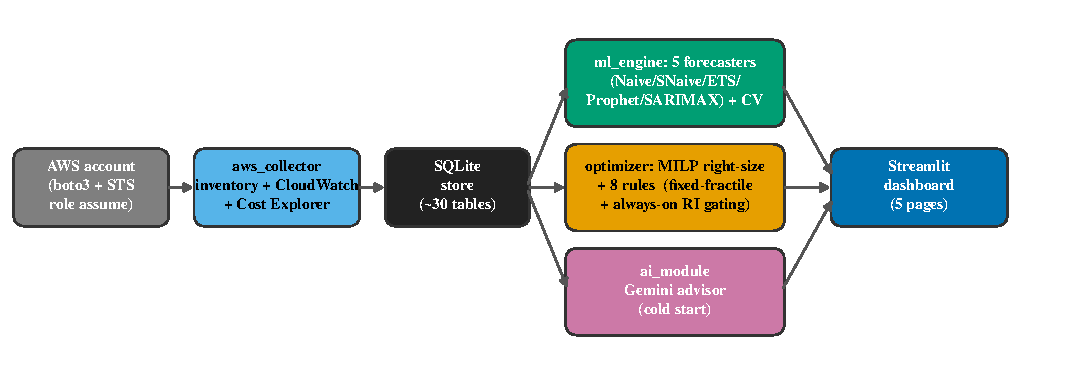
\includegraphics[width=0.96\textwidth]{fig_architecture.pdf}
\caption{System architecture. Telemetry is collected per AWS service, stored
in SQLite, and consumed by three engines---forecasting, the reservation
optimizer (MILP $+$ rules), and an LLM advisor---and surfaced in a dashboard.
The optimizer realizes the static core of the reservation policy of
Section~\ref{sec:model} (fixed-fractile sizing plus always-on reservation
gating); Section~\ref{sec:policysim} quantifies its distance from the
newsvendor/$(s,S)$ optimum.}
\label{fig:arch}
\end{figure*}

Fig.~\ref{fig:arch} shows the pipeline. A collection layer gathers inventory,
CloudWatch metrics, and Cost Explorer data for ten AWS resource types
(EC2/EBS, RDS, S3, Lambda, DynamoDB, ElastiCache, ECS, ELB, NAT) into a
per-account SQLite store; three engines then consume it.

\subsection{Forecasting the base demand distribution}
The forecasting engine implements five models behind one interface emitting
$[\textit{date},\textit{forecast},\textit{lower},\textit{upper}]$: a naive
last-value baseline, a seasonal-naive (weekly) baseline, additive
Holt--Winters exponential smoothing
(ETS)~\cite{winters1960holtwinters,hyndman2021fpp}, automatic seasonal ARIMA
(SARIMAX)~\cite{hyndman2008forecast}, and Prophet~\cite{taylor2018prophet}.
Models are compared by \emph{walk-forward (rolling-origin)
cross-validation}~\cite{tashman2000outofsample,bergmeir2012crossvalidation}:
an expanding training window of at least \cvInitial{} days, a step of
\cvStep{} days, and a forecast horizon $h$; accuracy is averaged over folds.
The selected model provides trend forecasts and prediction intervals for
monitoring; the empirical base distribution $\hat F_0$ used for sizing is
taken directly from the observed telemetry, and points exceeding
$\mu+2\sigma$ are flagged as surges (the realization of the state-1 / $d_1$
regime), in the spirit of streaming anomaly
detection~\cite{ahmad2017nab}.

\subsection{Sizing capacity with a MILP}
For compute (EC2, RDS) the optimizer solves a mixed-integer program with
CBC via PuLP~\cite{mitchell2011pulp}. Let $\mathcal{I}$ be the in-scope
instances, $\mathcal{C}$ the catalog of candidate types with price $p_c$,
vCPUs $v_c$, and memory $m_c$, and $x_{i,c}\in\{0,1\}$ assign type $c$ to
instance $i$:
\begin{align}
\min_{x}\;& \sum_{i\in\mathcal{I}}\sum_{c\in\mathcal{C}} p_c\,x_{i,c}
\label{eq:milp}\\
\text{s.t.}\;& \textstyle\sum_{c} x_{i,c}=1 && \forall i\in\mathcal{I},\nonumber\\
& \textstyle\sum_{c} v_c\,x_{i,c}\ge r_i^{\mathrm{cpu}} && \forall i,\nonumber\\
& \textstyle\sum_{c} m_c\,x_{i,c}\ge r_i^{\mathrm{mem}} && \forall i,\nonumber\\
& \textstyle\sum_{i}\sum_{c} p_c\,x_{i,c}\le B,\;\; x_{i,c}\in\{0,1\},\nonumber
\end{align}
where the capacity requirements $r_i^{\mathrm{cpu}},r_i^{\mathrm{mem}}$ are
the empirical fractiles of~\eqref{eq:p95} and $B$ is an optional budget cap
(left unbounded in our runs, so it does not shape the reported savings). The
memory constraint is imposed only for instances exposing a comparable
memory-utilization metric (EC2; omitted for RDS). The objective picks the
cheapest catalog type whose vCPU and memory cover the fractile-sized load:
this is the computational analogue of choosing $K_0$
in~\eqref{eq:fractiles}, with the residual tail $\pos{d-r_i}$ left to
on-demand spillover.

\subsection{Choosing reserved vs.\ on-demand, and removing waste}
Eight rule-based actions complete the policy (Algorithm~\ref{alg:pipe}). Two
\emph{pricing} rules realize the base-contract decision: an on-demand
resource with sufficient usage history is switched to a one-year reservation
when the reserved rate beats on-demand---i.e., committing the always-on base
capacity while leaving variable load on-demand. The pricing catalog's
one-year reserved rate is \rsvDiscountPct\% below on-demand
($\gamma\!\approx\!\rsvGamma$, and current AWS one-year standard
no-upfront pricing gives the same ratio, $\gamma\!\approx\!\extGammaReal$;
Section~\ref{sec:external}), so the reported reservation savings scale
roughly with $1-\gamma$. The remaining six target service-level waste:
EBS \texttt{gp2}$\rightarrow$\texttt{gp3} migration, deletion of
unattached/idle volumes and idle load balancers,
NAT-gateway$\rightarrow$VPC-endpoint replacement, S3 intelligent-tiering,
DynamoDB capacity-mode switching, and Lambda memory right-sizing. Each
action emits a per-resource saving
$\Delta_i=c_i^{\text{cur}}-c_i^{\text{new}}$; the engine de-duplicates by
$(\text{resource},\text{action})$ and persists the recommendations.

\begin{algorithm}[t]
\caption{Reservation-policy realization for one account}
\label{alg:pipe}
\begin{algorithmic}[1]
\Require account telemetry $\mathcal{D}$, catalog $\mathcal{C}$, budget $B$
\State \textsc{SelectModel}($\mathcal{D}$) \Comment{walk-forward CV; monitoring}
\State flag surges where cost $>\mu+2\sigma$ \Comment{state-1 demand}
\State $R \gets \emptyset$
\For{each compute service $s\in\{$EC2, RDS$\}$}
  \State $r_i \gets q_{0.95}(u_i)\,V_i\,h$ for $i\in\mathcal{I}_s$ \Comment{Eq.~\eqref{eq:p95}}
  \State $x^\star \gets$ solve MILP~\eqref{eq:milp} with $(r_i,B)$
  \State add right-size recs where $x^\star_i\neq$ current and cheaper
\EndFor
\For{each rule $\rho$ in the eight actions}
  \State $R \gets R \cup \rho(\mathcal{D})$ \Comment{reserved switch / waste removal}
\EndFor
\State de-duplicate $R$ by (resource, action); keep max saving
\State \Return $R$, $\sum_{r\in R}\Delta_r$
\end{algorithmic}
\end{algorithm}

A cold-start advisor (a large-language-model prompt over a nine-question
requirements form) covers accounts with no usage history; it is orthogonal
to the reservation policy and we do not evaluate its dollar impact here.

% =====================================================================
\section{Study I: Synthetic Account}\label{sec:eval}
% =====================================================================

\subsection{Setup and reproducibility}
Following the structure of~\cite[Sec.~7]{chen2024capacity}, we first fix the
workload, then evaluate forecasting and optimization. The workload is a
single representative account observed for \nDays{} days (\dataStart{} to
\dataEnd), spanning \numServicesBilled{} billed service categories and
\numResources{} resources (including \numEctwo{} EC2 instances). Daily cost
averages \$\meanDaily{} (standard deviation \$\stdDaily, range
\$\minDaily--\$\maxDaily), totaling \$\annualTotal{} over the year. Two
complementary bill views are used: a point-in-time resource-inventory bill
(\$\totalBill/month, the savings denominator) and this historical daily cost
series (\$\annualTotal/year). They differ by a few percent because the
former is a current snapshot of provisioned resources while the latter
integrates a year of daily charges, including transient resources; all
savings ratios use the inventory baseline. Defining a \emph{demand surge} as
a day exceeding $\mu+2\sigma=\$\surgeThresh$ isolates \numSurges{} pronounced
spikes (Fig.~\ref{fig:daily}); the largest reaches $z=\maxZ\sigma$ above the
mean. We read these spikes as the intermittent state-1 (surge) events of the
model; they recur irregularly across the year---the regime the reservation
policy is designed to handle. EC2 dominates the bill
(Fig.~\ref{fig:share}), so compute right-sizing and reservation carry the
largest savings potential. The workload is \emph{synthetic}, modeled on
public cloud traces~\cite{shen2015bitbrains,ahmad2017nab};
Section~\ref{sec:external} repeats the transferable parts of the study on
real telemetry.

\emph{Reproducibility.} Every number, table cell, and figure in
Sections~\ref{sec:eval}--\ref{sec:policysim} is emitted as a \LaTeX{} macro
by four scripts in five invocations (\texttt{make\_figures.py},
\texttt{external\_validation.py}, \texttt{azure\_validation.py}, and
\texttt{policy\_sim.py} on two inputs)
from the account database, the public traces (fetched by a pinned script
from the archive maintainers' mirror), and a snapshot-dated price catalog.
Stochastic components are seeded; we verify by running the chain twice in
the pinned environment and diffing every generated artifact.

\begin{figure*}[t]
\centering
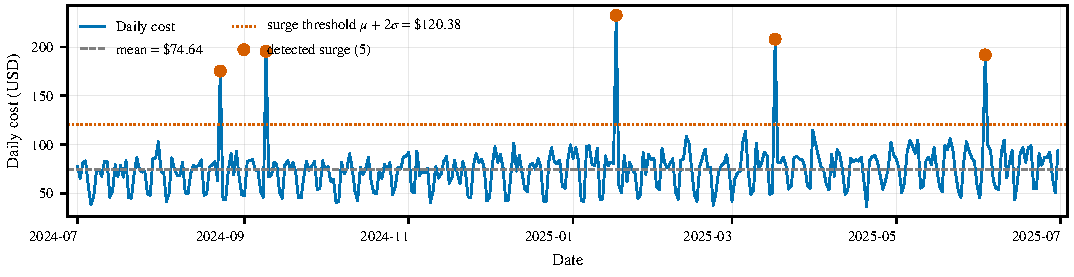
\includegraphics[width=0.96\textwidth]{fig_daily_surges.pdf}
\caption{Daily cost over \nDays{} days (synthetic account). The dotted line
is the surge threshold $\mu+2\sigma=\$\surgeThresh$; \numSurges{} days
(markers) exceed it. Base demand is stationary around \$\meanDaily/day;
surges are intermittent and large.}
\label{fig:daily}
\end{figure*}

\begin{figure}[t]
\centering
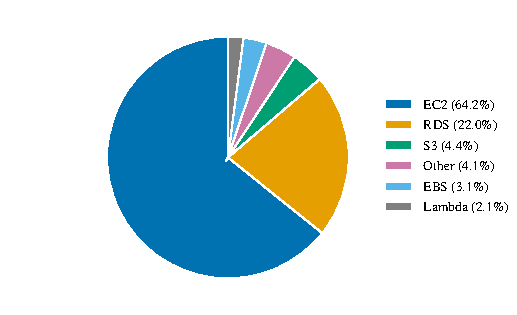
\includegraphics[width=0.8\columnwidth]{fig_service_share.pdf}
\caption{Study I: share of the monthly bill by service category (Cost
Explorer buckets; non-itemized services fold into ``Other''). EC2 dominates,
so compute right-sizing and reservation carry the largest savings.}
\label{fig:share}
\end{figure}

\subsection{Forecasting performance}\label{sec:eval:forecast}
Table~\ref{tab:mape} and Fig.~\ref{fig:mape} report walk-forward mean
absolute percentage error (MAPE, mean$\pm$sd across folds) by model and
horizon; at the deployment-relevant $30$-day horizon we additionally report
the mean absolute scaled error (MASE)~\cite{hyndman2006mase} and
$95\%$-interval coverage. Exponential smoothing (ETS) has the best mean at
$30$ days (\mapeEts\%$\pm$\mapeSdEts) and the best MASE (\maseEts{} vs.\
\maseSnaive{} for seasonal-naive; both beat the in-sample seasonal-naive
benchmark of $1.0$), and its accuracy is far more stable across folds
(sd \mapeSdEts{} vs.\ \mapeSdSnaive). However, the point-accuracy difference
between ETS and the seasonal-naive baseline is \emph{not statistically
significant} at this sample size: a Diebold--Mariano test with the
Harvey--Leybourne--Newbold small-sample
correction~\cite{diebold1995comparing,harvey1997testing} on the pooled
$1$--$30$-step-ahead errors (\nFoldsThirty{} contiguous, non-overlapping
test windows; autocovariance truncation at lag $h{-}1$) gives
$\mathrm{DM}=\dmStatEtsSnaive$, $p=\dmPEtsSnaive$, and a Wilcoxon
signed-rank test on per-fold MAPEs gives $p=\wilcoxonPEtsSnaive$. We
therefore claim model \emph{selection}, not model \emph{superiority}: ETS is
selected for its stability, MASE, and conservative, over-covering intervals
(\covEts\% empirical coverage vs.\ nominal $95\%$---over-wide but safe for
capacity work, unlike Prophet's severe under-coverage at \covProphet\%),
consistent with guidance on comparing few models over short evaluation
windows~\cite{diebold2015comparing,hewamalage2023forecast}. Prophet trails on accuracy
(\mapeProphet\%$\pm$\mapeSdProphet{} at $30$ days)---its yearly-seasonality
components overfit a single year of data---and the naive baseline
(\mapeNaive\%) confirms the series is non-trivial.

Fig.~\ref{fig:holdout} shows the selected model's $30$-day holdout forecast
with a $95\%$ interval: ETS tracks the base load at \holdoutMape\% MAPE with
\holdoutCov\% empirical interval coverage, but the lone in-window surge
pierces the upper band. This is consistent with the policy's premise: on
this workload the base process does not anticipate the surge, so the surge
is the spillover the reservation policy routes to on-demand rather than
provisioning reserved capacity against. Because the workload is synthetic
with injected spikes, we read this as confirming a modeling assumption, not
as evidence that real-world surges are inherently unforecastable.

\begin{table}[t]
\caption{Study I: walk-forward MAPE (\%, mean $\pm$ sd across folds) by model
and horizon (days). Best mean per column in bold. Expanding window, initial
\cvInitial{} days, step \cvStep{} days.}
\label{tab:mape}
\centering
\renewcommand{\arraystretch}{1.15}
\setlength{\tabcolsep}{3pt}%
\resizebox{\columnwidth}{!}{%
\begin{tabular}{@{}l r r r r r @{}}
\toprule
Model & $h{=}7$ & $h{=}14$ & $h{=}30$ & $h{=}60$ & $h{=}90$ \\
\midrule
ETS (selected)   & 11.28 $\pm$ 2.54 & 11.24 $\pm$ 2.45 & \textbf{11.20 $\pm$ 0.57} & \textbf{11.39 $\pm$ 0.74} & \textbf{12.15 $\pm$ 2.39} \\
SeasonalNaive    & \textbf{10.18 $\pm$ 2.84} & \textbf{10.84 $\pm$ 2.75} & 12.28 $\pm$ 2.82 & 12.66 $\pm$ 2.21 & 12.91 $\pm$ 2.02 \\
Prophet          & 14.41 $\pm$ 6.22 & 20.47 $\pm$ 7.40 & 20.93 $\pm$ 7.53 & 19.70 $\pm$ 7.89 & 18.08 $\pm$ 8.42 \\
Naive            & 25.16 $\pm$ 4.47 & 27.90 $\pm$ 3.52 & 27.26 $\pm$ 4.36 & 27.87 $\pm$ 4.09 & 27.38 $\pm$ 3.70 \\
\bottomrule
\end{tabular}}

\end{table}

\begin{figure}[t]
\centering
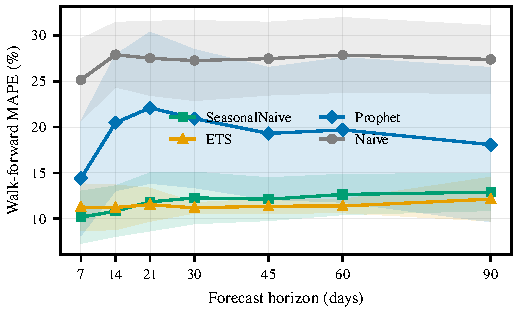
\includegraphics[width=\columnwidth]{fig_mape_horizon.pdf}
\caption{Study I: walk-forward MAPE vs.\ horizon (shaded bands: $\pm1$ sd
across folds). ETS has the best mean at $h\ge30$ days and the smallest
fold-to-fold sd; seasonal-naive wins at short horizons, and their difference
is not statistically significant (Section~\ref{sec:eval:forecast}). Both
beat the naive baseline. SARIMAX is excluded for runtime (minutes per
fold).}
\label{fig:mape}
\end{figure}

\begin{figure}[t]
\centering
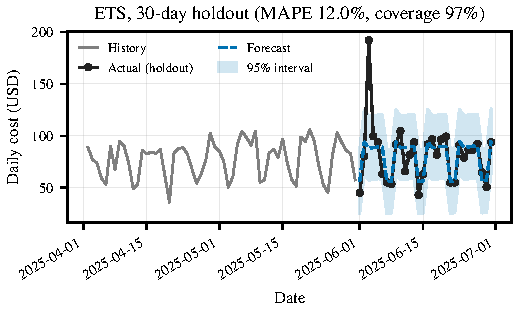
\includegraphics[width=\columnwidth]{fig_forecast_holdout.pdf}
\caption{Study I: ETS $30$-day holdout forecast with $95\%$ interval. The
base load is tracked at \holdoutMape\% MAPE; the single surge exceeds the
band (on-demand spillover).}
\label{fig:holdout}
\end{figure}

\subsection{Optimization savings}
The optimizer produces \numRecs{} recommendations (plus \numAiRecs{}
advisory items). Summed independently they total \$\totalSavings/month;
because \numOverlap{} EBS volumes are flagged for both deletion and a
\texttt{gp3} upgrade, the jointly-realizable total after de-duplication is
\$\jointSavings/month (the \$\overlapSavings{} difference is the only
double-counted amount). Against the \$\totalBill/month inventory bill the
additive figure is a \savingsPctBill\% reduction (upper bound), taking
monthly spend to \$\billAfter; on the \$\flaggedCost{} of resources flagged,
the upper-bound reduction is \savingsPctFlagged\%.
Fig.~\ref{fig:savings} breaks the savings down by action. Two compute levers
dominate and, crucially, target \emph{disjoint} resources---MILP
right-sizing of over-provisioned RDS databases (\$\savRightsize,
\cntRightsize{} recs) and the reserved/pricing switch on always-on EC2
instances (\$\savPricing, \cntPricing{} recs)---so their combined
\$\savComputeTwo{} ($\pctComputeTwo\%$ of the total) is fully jointly
realizable. The six waste-removal rules contribute the long tail. On this
EC2/RDS-heavy account the dominance of the two compute levers reflects the
workload composition---a few large over-provisioned and always-on
instances---rather than a theorem; it is consistent with the policy's
emphasis on sizing base capacity correctly. By confidence, \cntHigh{}
high-confidence recommendations carry \$\savHigh, \cntMed{}
medium-confidence ones \$\savMed, and \cntLow{} low-confidence ones
\$\savLow.

\begin{figure}[t]
\centering
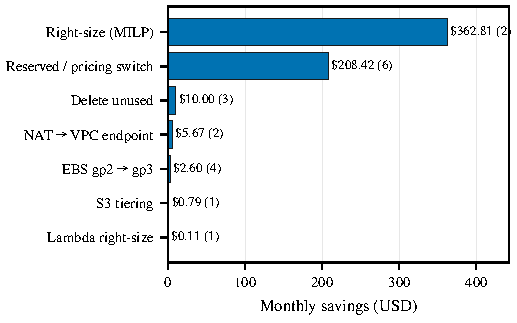
\includegraphics[width=\columnwidth]{fig_savings_breakdown.pdf}
\caption{Study I: recommended monthly savings by optimization action (USD;
recommendation count in parentheses). Right-sizing and the reserved/pricing
switch dominate.}
\label{fig:savings}
\end{figure}

% =====================================================================
\section{Study II: External Validation on Real Traces}\label{sec:external}
% =====================================================================
Study I establishes the pipeline on a workload whose ground truth we
control; this section validates the transferable parts on \emph{real}
telemetry from two managed-hosting providers, and reports honestly where
reality is harder than the synthetic account.

\subsection{Traces, cost model, and protocol}
We use three public per-VM datasets: \textbf{fastStorage}
(\extFsVms{} VMs, one month, August 2013) and \textbf{Rnd} (\extRndVms{}
VMs, three months) from the Bitbrains GWA-T-12 trace of business-critical
enterprise workloads~\cite{shen2015bitbrains,iosup2008gwa}, and
\textbf{Materna-Trace-3} (\extMatVms{} VMs, 2016) from the Materna GWA-T-13
trace. Each VM reports, at $300$-second sampling, its provisioned cores,
CPU capacity (MHz), memory capacity, and CPU/memory usage. These are the
same traces our synthetic workload was modeled on, which makes them the
natural external check; they are also among the few public traces exposing
both provisioned capacity \emph{and} usage per VM at this granularity (the
Azure and Google traces bucket or omit provisioned
memory~\cite{cortez2017resource,tirmazi2020borgng}, and the Alibaba traces
report container-level, normalized
usage~\cite{lu2017imbalance,guo2019alibaba}).

\emph{Cost model.} We price VMs against a \extCatalogSize-type AWS
\texttt{us-east-1} Linux catalog (t3/m5/c5/r5 families) whose on-demand and
one-year standard no-upfront reserved rates were extracted from AWS's Price
List bulk file (snapshot \extSnapshot) and cross-checked against two
independent sources; the implied reserved ratio is
$\gamma=\extGammaReal$. The \emph{baseline} is a like-for-like
lift-and-shift: each VM is assigned the cheapest type covering its
\emph{provisioned} cores and memory---the migration a team performs when it
does not right-size. The \emph{optimized} assignment solves the system's own
MILP~\eqref{eq:milp} with requirements from the deployed
rule~\eqref{eq:p95}: the $95$th percentile of observed CPU (and memory)
usage with $1.3\times$ headroom. No VM exceeded the largest catalog type
(\extFsClamped{} clamped). Without a budget cap the integer program
decomposes into independent per-VM cheapest-covering choices, so this study
exercises the system's requirement definitions and implementation rather
than the coupled, budget-constrained program.

\subsection{Right-sizing results}
Table~\ref{tab:ext} summarizes. On fastStorage the MILP cuts the baseline
bill from \$\extFsBaseline/month to \$\extFsOptimized/month
(\textbf{\extFsSavingsPct\%}), down-sizing \extFsDownsized{} VMs while
\emph{up}-sizing \extFsUpsized{} genuinely under-provisioned ones (the rule
is not a pure cost cutter; it also fixes performance risks). The independent
Rnd dataset gives a nearly identical relative saving
(\extRndSavingsPct\%)---evidence the result is a property of the method
rather than of one dataset---and Materna, a far more over-provisioned
infrastructure, yields \extMatSavingsPct\%. Because trace VMs are always-on,
the reservation lever applies on top: pricing the optimized fleet at
one-year reserved rates yields total reductions of \extFsSavingsPctRi\%,
\extRndSavingsPctRi\%, and \extMatSavingsPctRi\% respectively. The
magnitudes are consistent with published production experience: at Google,
autopiloted jobs run at $23\%$ slack versus $46\%$ for manually-managed
ones~\cite{rzadca2020autopilot}, and a recent SAP production trace finds
the large majority of VMs using well under their
provisioning~\cite{uhlig2025sap}.

\subsection{Scale, and a boundary condition: a 237k-VM Azure fleet}
\label{sec:ext:azure}
To probe scale and era, we repeat the right-sizing analysis on the Azure
Public Dataset V2 (2019 production trace from the Resource Central
repository~\cite{cortez2017resource}): of \azTotalRows{} VMs, \azVms{}
survive the filters (lifetime $\ge7$ days---most Azure VMs are
short-lived---plus numeric capacity buckets and a valid $p_{95}$ reading;
the \azDroppedBucket{} VMs in the unpublishable ``$>$24-core/$>$64-GB''
buckets are the trace's largest), and for each Azure publishes provisioned
core/memory \emph{buckets} and the $95$th percentile of five-minute
\emph{maximum} CPU readings. Two semantics therefore differ from the Bitbrains/Materna study:
utilization percentiles are max-based rather than mean-based, and---since
no memory-usage series is published---memory is held at its provisioned
bucket (never downsized). The result is an instructive \emph{negative}:
right-sizing alone is cost-negative (\azSavingsPct\%; \azDownsized{} VMs
down-sized but \azUpsized{} up-sized, since any VM with max-based
$p_{95}$ above $77\%$ exceeds its provisioned cores under the $1.3\times$
headroom), even though the fleet carries $53\%$ aggregate CPU slack that
the memory floor and hot maxima make unreachable. The reservation lever,
by contrast, still yields \azSavingsPctRi\% on the same fleet---net of the
right-sizing loss (reserved pricing alone saves $1{-}\gamma$ on an
always-on fleet). The reading
is a boundary condition for the deployed rule, invisible on traces that
publish usage means: the fractile heuristic's value is contingent on the
\emph{semantics} of the utilization metric and on which resources are
measurable, whereas the $\gamma$-driven pricing lever is robust across all
four datasets.

\begin{table}[t]
\caption{Study II: right-sizing real VMs with the system's MILP against a
like-for-like lift-and-shift baseline, priced at AWS on-demand rates
(snapshot \extSnapshot); the last column additionally applies one-year
reserved-instance (RI) pricing ($\gamma=\extGammaReal$) to the optimized
fleet.}
\label{tab:ext}
\centering
\renewcommand{\arraystretch}{1.15}
\setlength{\tabcolsep}{4pt}
\begin{tabular}{@{}l r r r r r@{}}
\toprule
Dataset & VMs & Baseline & Optimized & Saving & $+$RI \\
 & & (\$/mo) & (\$/mo) & (\%) & (\%) \\
\midrule
Bitbrains fastStorage & \extFsVms  & \extFsBaseline  & \extFsOptimized  & \extFsSavingsPct  & \extFsSavingsPctRi \\
Bitbrains Rnd         & \extRndVms & \extRndBaseline & \extRndOptimized & \extRndSavingsPct & \extRndSavingsPctRi \\
Materna-Trace-3       & \extMatVms & \extMatBaseline & \extMatOptimized & \extMatSavingsPct & \extMatSavingsPctRi \\
\bottomrule
\end{tabular}
\end{table}

\subsection{Forecasting real aggregate demand is hard}\label{sec:ext:forecast}
We repeat the walk-forward protocol of Section~\ref{sec:eval:forecast} on
the Rnd cluster's aggregate CPU demand (\extRndHours{} hourly points over
three months, mean \extRndMeanGhz~GHz; Fig.~\ref{fig:extseries}), at its
native hourly scale (season $24$, horizons $6$--$48$\,h) and, aligned with
Study I, on the daily aggregate (horizons $7$/$14$\,d).
Table~\ref{tab:extmape} reports the results, and they are sobering: the best
hourly model reaches only \extBestMape\% MAPE at $24$\,h
(\extBestModel), the best daily model \extDailyBestMape\% at $7$\,d
(\extDailyBestModel), and none of the tested pairs is statistically
separable (ETS vs.\ seasonal-naive DM $p=\extDmP$; Prophet vs.\
seasonal-naive $p=\extDmPProphetSnaive$; Prophet vs.\ naive
$p=\extDmPProphetNaive$; all at $24$\,h). The
MASE values tell the structural story: all models sit near $1.0$
(\extMaseNaive--\extMaseSnaive{} at $24$\,h), i.e.\ none meaningfully beats
a naive benchmark, and seasonal-naive is \emph{worse} than plain naive
(MASE \extMaseSnaive{} vs.\ \extMaseNaive)---this aggregate is dominated by
irregular regime shifts rather than stable daily seasonality, and
\extRndSurges{} of \extRndHours{} hours sit above the $\mu+2\sigma$ surge
threshold. ETS interval coverage collapses to \extCovEts\% (nominal
$95\%$). We report this as a finding, not a failure: it is precisely the
regime in which point-forecast-driven provisioning is fragile, and it
motivates the design in which capacity is sized from the \emph{empirical
demand distribution} (quantiles, Section~\ref{sec:policysim}) while point
forecasts serve the softer roles of trend reporting and anomaly context.

\begin{figure*}[t]
\centering
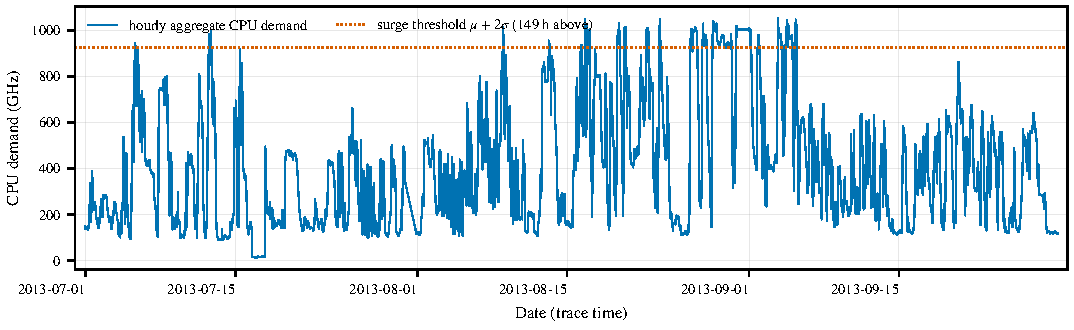
\includegraphics[width=0.82\textwidth]{fig_ext_series.pdf}
\caption{Study II: hourly aggregate CPU demand of the Bitbrains Rnd cluster
(\extRndVms{} VMs, three months). \extRndSurges{} hours exceed the
$\mu+2\sigma$ surge threshold; the series exhibits irregular regime shifts
rather than stable seasonality.}
\label{fig:extseries}
\end{figure*}

\begin{table}[t]
\caption{Study II: walk-forward MAPE (\%, mean $\pm$ sd across folds) on the
real Rnd aggregate, at hourly (left) and daily (right) granularity. Best
mean per column in bold. No tested pairwise difference is statistically
significant (Section~\ref{sec:ext:forecast}).}
\label{tab:extmape}
\centering
\renewcommand{\arraystretch}{1.15}
\setlength{\tabcolsep}{3pt}
\resizebox{\columnwidth}{!}{%
\begin{tabular}{@{}l r r r r r r @{}}
\toprule
Model & $h{=}6$\,h & $h{=}12$\,h & $h{=}24$\,h & $h{=}48$\,h & $h{=}7$\,d & $h{=}14$\,d \\
\midrule
ETS            & \textbf{48.2 $\pm$ 46.2} & 71.9 $\pm$ 55.4 & 77.0 $\pm$ 57.2 & 91.2 $\pm$ 47.8 & \textbf{52.1 $\pm$ 29.9} & 64.4 $\pm$ 40.9 \\
SeasonalNaive  & 65.9 $\pm$ 33.6 & 73.7 $\pm$ 46.3 & 65.0 $\pm$ 40.3 & \textbf{65.8 $\pm$ 33.8} & 54.2 $\pm$ 22.6 & \textbf{59.7 $\pm$ 32.9} \\
Prophet        & 49.0 $\pm$ 26.2 & \textbf{60.5 $\pm$ 30.0} & \textbf{60.8 $\pm$ 21.6} & 88.1 $\pm$ 42.3 & 59.8 $\pm$ 36.9 & 66.7 $\pm$ 30.0 \\
Naive          & 57.4 $\pm$ 71.2 & 87.9 $\pm$ 86.1 & 82.3 $\pm$ 66.6 & 94.2 $\pm$ 55.7 & 53.4 $\pm$ 14.2 & 66.5 $\pm$ 44.5 \\
\bottomrule
\end{tabular}}

\end{table}

% =====================================================================
\section{Study III: The Price of Conservatism}\label{sec:policysim}
% =====================================================================
Sections~\ref{sec:eval}--\ref{sec:external} evaluated the system as built.
This section asks the converse question: \emph{what would the theory of
Section~\ref{sec:model} be worth if the sizing fractile followed it?} We
answer with an out-of-sample policy simulation on both workloads.

\subsection{Protocol}
Demand is the daily cost series of Study I (\polTrainDays{} training days,
\polTestDays{} test days) and the hourly Rnd aggregate of Study II
(\extPolTrainDays{} training hours, \extPolTestDays{} test hours), split
chronologically $60/40$; every policy sets its capacity from the training
split only and is charged on the test split. One exception is flagged
explicitly: DUAL assumes the surge \emph{state} is observable during
execution (the information structure of the state-modulated
model~\cite{chen2024capacity}), so we also report DUALC, a causal variant
with no contemporaneous knowledge. Costs follow the average-cost
model~\eqref{eq:ac} in units of the on-demand rate: static reserved capacity
$K$ costs $\gamma K + \E\pos{D-K}$ per period, so no price catalog is needed
and results are reported as a percentage of the \emph{on-demand-only}
baseline. We sweep $\gamma\in[0.50,0.95]$ and highlight
$\gamma^{*}{=}\polGammaStar$, the ratio of both our catalog and current AWS
one-year pricing (Sections~\ref{sec:system}--\ref{sec:external}). Seven
policies compete:

\begin{itemize}
\item \textbf{OD}: on-demand only ($K{=}0$); the normalization baseline.
\item \textbf{HEUR}: the deployed fractile rule~\eqref{eq:p95} read as a
reservation-sizing policy, $K = q_{0.95}(D_{\mathrm{train}})\times 1.3$. On
these workloads this covers the \polImpliedQ th (synthetic) and
\extPolImpliedQ th (trace) percentile of training demand.
\item \textbf{NV}: the newsvendor optimum of Remark~\ref{rem:service}, the
empirical $(1{-}\gamma)$ training quantile---the data-driven newsvendor
estimator~\cite{arrow1951inventory,ban2019newsvendor}.
\item \textbf{SAA}: a two-stage stochastic program (first stage: $K$; second
stage: per-scenario spillover) solved by sample-average approximation over
the training periods with the same PuLP/CBC toolchain as the system's MILP;
this is the classical SP formulation of cloud reservation
\cite{chaisiri2012provisioning,bulbul2021provisioning} serving as an
independent baseline.
\item \textbf{DUAL}: the dual-capacity $(K_0,K_1)$ SAA of~\eqref{eq:ac},
with surge periods labeled by the training $\mu+2\sigma$ threshold; base
capacity $K_0$ is always reserved, supplementary $K_1-K_0$ only during
surges. This is a static step toward the $(s,S)$ supplementary-contract
dynamics of~\cite{chen2024capacity}; because it assumes the surge state is
observable at execution time, it is an upper bound on implementable value.
\item \textbf{DUALC}: the same $(K_0,K_1)$ contracts activated
\emph{causally}---the supplementary tier is on in period $t$ iff period
$t{-}1$ exceeded the surge threshold. No contemporaneous knowledge.
\item \textbf{LB}: a clairvoyant lower bound, $\gamma\,\E[D_{\mathrm{test}}]$
(reserve exactly the realized demand each period; ignores commitment
inflexibility).
\end{itemize}

Table~\ref{tab:fractile} restates the analytical gap the simulation
quantifies: across realistic discounts the deployed fractile ($0.95$) sits
far above the cost-optimal $1-\gamma$.

\begin{table}[t]
\caption{Cost-optimal reserved service level $1-\gamma$ vs.\ the deployed
$q{=}0.95$ heuristic, by reserved/on-demand ratio $\gamma=w_T/w_0$.}
\label{tab:fractile}
\centering
\renewcommand{\arraystretch}{1.15}
\begin{tabular}{@{}l c c c c@{}}
\toprule
$\gamma=w_T/w_0$ & 0.60 & 0.70 & 0.80 & 0.90 \\
\midrule
optimal fractile $1-\gamma$ & 0.40 & 0.30 & 0.20 & 0.10 \\
deployed fractile $q$       & 0.95 & 0.95 & 0.95 & 0.95 \\
\bottomrule
\end{tabular}
\end{table}

\subsection{Results}
Fig.~\ref{fig:policy} (synthetic) and Fig.~\ref{fig:policyext} (real trace)
plot realized test cost against $\gamma$;
Tables~\ref{tab:policy}--\ref{tab:policyext} tabulate four discount levels.
Four findings:

\textbf{F1 --- the conservative fractile forfeits the discount.} At
$\gamma^{*}{=}\polGammaStar$, HEUR realizes \polPctHeur\% of the on-demand
baseline on the synthetic account and \extPolPctHeur\% on the real
trace---at and beyond break-even. Reserving to the
\polImpliedQ th--\extPolImpliedQ th percentile of a skewed demand
distribution commits far more capacity than the mean demand uses: on the
synthetic account HEUR crosses break-even at
$\gamma\approx\polHeurBreakeven$, and on the trace it exceeds the on-demand
bill across the entire sweep. In
dollars, on the synthetic account the rule would pay
\$\polHeurMonthly/month against \$\polOdMonthly{} on-demand, while the
newsvendor fractile pays \$\polNvMonthly---a \$\polPoCMonthly/month
\emph{price of conservatism} (\polPoC{} percentage points; \extPolPoC{}
points on the trace). We emphasize the framing: the deployed \emph{system}
does not size reservations this way---it right-sizes instance types
with~\eqref{eq:p95} and gates the reservation switch on always-on usage
(Section~\ref{sec:system})---and F1 is precisely the quantitative reason
that design choice is correct. F1 is thus a cautionary out-of-sample bound
on naively transferring the right-sizing fractile to commitment sizing---a
transfer that is tempting precisely because the percentile idiom is
standard for capacity limits~\cite{rzadca2020autopilot,cortez2017resource},
while commercial commitment recommenders instead maximize savings over
replayed historical usage~\cite{awsri2026,awssp2026,azureres2026}; F1
quantifies why that is the right instinct.

\textbf{F2 --- the newsvendor fractile is robust out of sample.} NV
realizes \polPctNv\% (synthetic) and \extPolPctNv\% (trace) of the
on-demand baseline at $\gamma^{*}$---a \polNvSave\%/\extPolNvSave\% saving
from a one-line, distribution-free rule---even though the trace's test
window is substantially surgier than its training window
(\extPolSurgeTest{} vs.\ \extPolSurgeTrain{} surge hours under the
training-split threshold; the full-series threshold of
Section~\ref{sec:external} flags \extRndSurges). The ordering is
insensitive to the split choice: across train fractions $0.5$--$0.7$ the
newsvendor saving stays within \polNvSaveMin--\polNvSaveMax\% (synthetic)
and \extPolNvSaveMin--\extPolNvSaveMax\% (trace).

\textbf{F3 --- the two-tier structure pays exactly when surge states
persist.} DUAL improves on NV by only \polDualGain{} points on the
tame synthetic series (\polPctDual\% vs.\ \polPctNv\%) but by
\extPolDualGain{} points on the real trace (\extPolPctDual\% vs.\
\extPolPctNv\%): the base commitment stays at the newsvendor level
($K_0{=}\polKdualbase$ vs.\ single $K{=}\polKnv$ \$/day on the synthetic
account) while a supplementary tier ($K_1{=}\polKdualsurge$) is paid for
only during surge periods---capacity a single static $K$ must either
commit to permanently or forgo. DUAL's observable-state assumption makes
it an upper bound; the causal variant tells the sharper story. On the real
trace, where surge episodes persist across hours, activating on the
previous hour's signal retains nearly all of the value (DUALC
$+\extPolDualcGain$ of the $+\extPolDualGain$ points); on the synthetic
account, whose surges are isolated single days, DUALC arrives a day late
and realizes \polPctDualc\%---\emph{worse} than NV. Surge persistence, not
burstiness alone, is the enabling condition. On the trace the finding is
robust to the labeling threshold (sweeping $\mu{+}k\sigma$,
$k\in\{1.5,2,2.5\}$, the causal gain stays positive at
\extPolDualcGainThreshMin--\extPolDualcGainThreshMax{} points) and degrades
gracefully under contract-term friction: with contracts sized ignoring the
term constraint, a minimum supplementary term of
$6$ or $24$ hours reduces the causal gain to \extPolDualcGainHoldSix{} and
\extPolDualcGainHoldDay{} points, while a week-long minimum term destroys
it (\extPolDualcGainHoldWeek)---quantifying, on real demand, why the
cancellation flexibility at the heart of~\cite{chen2024capacity} matters.
This is, to our knowledge,
the first out-of-sample quantification of the value of the
base/supplementary contract structure of~\cite{chen2024capacity} on real
cloud telemetry, and it supports implementing the full $(s,S)$ dynamics as
the highest-value system extension.

\textbf{F4 --- the SP baseline recovers the closed form.} The SAA program's capacity matches the newsvendor
quantile to within \polSaaNvGapPct\% (synthetic) and \extPolSaaNvGapPct\%
(trace) across the sweep---as theory requires, since SAA of the same
empirical distribution optimizes the same objective---which cross-validates
the closed-form policy, our simulator, and the SP implementation, and
confirms that nothing here hinges on solver choice. Because savings
maximization over replayed historical usage is also the computation
commercial recommenders document~\cite{awsri2026,awssp2026,azureres2026},
F4 doubles as an indirect validation of that practice: replay-and-maximize
recovers the newsvendor optimum, and both differ sharply from
fractile-based sizing (F1).

\begin{figure}[t]
\centering
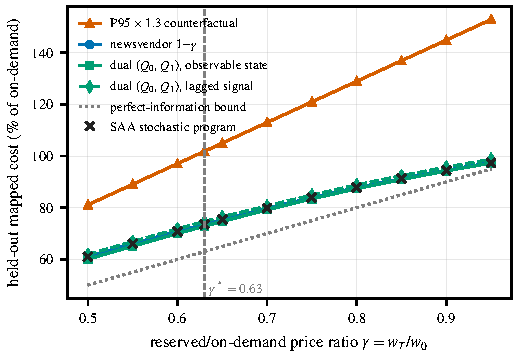
\includegraphics[width=\columnwidth]{fig_policy_gamma.pdf}
\caption{Study III (synthetic account): realized out-of-sample cost, as \% of
on-demand-only, vs.\ reserved discount $\gamma$. The deployed
$q{=}0.95{\times}1.3$ fractile read as reservation sizing crosses break-even
at $\gamma\approx\polHeurBreakeven$; the newsvendor fractile and its SAA
twin track the clairvoyant bound.}
\label{fig:policy}
\end{figure}

\begin{figure}[t]
\centering
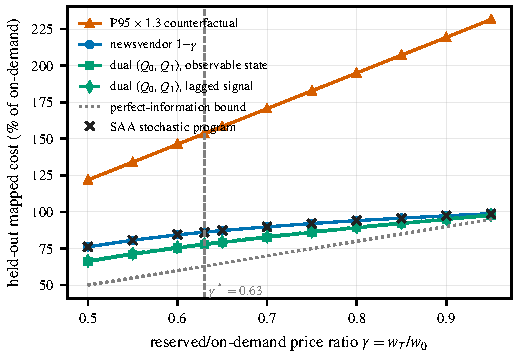
\includegraphics[width=\columnwidth]{fig_policy_gamma_ext.pdf}
\caption{Study III (real Bitbrains Rnd demand): realized out-of-sample cost,
as \% of on-demand-only, vs.\ reserved discount $\gamma$ (cf.\
Fig.~\ref{fig:policy}). On real demand with persistent surges both
dual-capacity variants open a clear gap over single-capacity newsvendor
sizing.}
\label{fig:policyext}
\end{figure}

\begin{table}[t]
\caption{Study III (synthetic): realized test cost as \% of on-demand-only,
by policy and reserved discount $\gamma$. Bold: best among policies
requiring no contemporaneous surge-state knowledge (the observable-state
dual and the clairvoyant bound are excluded from bolding).}
\label{tab:policy}
\centering
\renewcommand{\arraystretch}{1.15}
\setlength{\tabcolsep}{4pt}
\begin{tabular}{@{}l r r r r @{}}
\toprule
Policy & $\gamma{=}0.60$ & $\gamma{=}0.70$ & $\gamma{=}0.80$ & $\gamma{=}0.90$ \\
\midrule
P95 $\times$ 1.3 counterfactual & 97.0 & 113.0 & 128.9 & 144.9 \\
newsvendor $1{-}\gamma$ & 70.8 & 79.7 & 87.7 & 94.5 \\
SAA stochastic program & 70.8 & 79.8 & 87.8 & 94.5 \\
7-day recency-window replay & 71.0 & 80.2 & 87.6 & 94.5 \\
30-day recency-window replay & \textbf{70.5} & \textbf{79.7} & \textbf{87.4} & \textbf{94.3} \\
60-day recency-window replay & 70.5 & 79.8 & 87.5 & 94.6 \\
dual $(Q_0,Q_1)$, obs.\ state & 70.0 & 79.2 & 87.3 & 94.2 \\
dual $(Q_0,Q_1)$, lagged signal & 71.8 & 80.6 & 88.8 & 95.7 \\
perfect-information bound & 60.0 & 70.0 & 80.0 & 90.0 \\
\bottomrule
\end{tabular}

\end{table}

\begin{table}[t]
\caption{Study III (real Bitbrains Rnd demand): realized test cost as \% of
on-demand-only, by policy and reserved discount $\gamma$ (cf.\
Table~\ref{tab:policy}).}
\label{tab:policyext}
\centering
\renewcommand{\arraystretch}{1.15}
\setlength{\tabcolsep}{4pt}
\begin{tabular}{@{}l r r r r @{}}
\toprule
Policy & $\gamma{=}0.60$ & $\gamma{=}0.70$ & $\gamma{=}0.80$ & $\gamma{=}0.90$ \\
\midrule
P95 $\times$ 1.3 counterfactual & 146.2 & 170.6 & 195.0 & 219.3 \\
newsvendor $1{-}\gamma$ & 84.4 & 89.8 & 94.1 & 97.4 \\
SAA stochastic program & 84.4 & 89.8 & 94.1 & 97.4 \\
7-day recency-window replay & 89.3 & 95.6 & 102.4 & 103.6 \\
30-day recency-window replay & 82.7 & 89.2 & 93.8 & 97.3 \\
60-day recency-window replay & 84.4 & 89.8 & 94.1 & 97.4 \\
dual $(Q_0,Q_1)$, obs.\ state & 75.4 & 82.7 & 89.2 & 94.9 \\
dual $(Q_0,Q_1)$, lagged signal & \textbf{75.8} & \textbf{83.1} & \textbf{89.6} & \textbf{95.3} \\
perfect-information bound & 60.0 & 70.0 & 80.0 & 90.0 \\
\bottomrule
\end{tabular}

\end{table}

\subsection{Implications for the deployed system}
The simulation prescribes three concrete changes, in decreasing order of
value. First, any lever that sizes \emph{commitments} should use the
$\gamma$-aware newsvendor fractile $1-\gamma$, not a fixed high percentile;
the required inputs (the reserved ratio and the empirical demand
distribution) are already in the system's database. Second, for workloads
with persistent surges the base/supplementary split is worth
implementing---on real demand the observable-state policy captured
\extPolDualGapCapture\% of the remaining gap between NV and the clairvoyant
bound, and the causal activation rule retained
\extPolDualcGapCapture\%---which is the static core of the reference's
$(s,S)$ policy; the dynamic cancellation/renewal thresholds remain future
work.
Third, the fixed $q{=}0.95{\times}1.3$ rule remains appropriate where it is
actually deployed (sizing instance types against performance risk); the
system's separation of concerns---percentile for capacity, always-on gating
for commitment---is validated by F1.

% =====================================================================
\section{Threats to Validity}\label{sec:threats}
% =====================================================================
\textbf{Workload provenance.} Study I uses a synthetic, single-account
dataset that ships with the system; its dollar figures are
method-illustrative, not measured savings on production infrastructure.
Study II mitigates this with real telemetry, but from two providers with
traces collected in 2013 (Bitbrains) and 2016 (Materna), each spanning one
to three months; modern cloud usage is burstier and more
heterogeneous~\cite{tirmazi2020borgng}, which plausibly \emph{strengthens}
the case for surge-aware policies (F3) but is untested here; the Azure arm
(2019) is newer but bucketed. Validation on a post-2019 per-VM trace
(e.g.,~\cite{uhlig2025sap}) and on a live account remain open.

\textbf{Trace cost model.} Study II prices 2013--2019 VMs at 2026 AWS rates
under a like-for-like mapping (cheapest type covering provisioned
capacity), ignores licensing, storage, network egress, and sustained-use or
negotiated discounts, and assumes VMs are always-on when applying reserved
rates (true for the trace populations studied). The baseline is a
\emph{naive} lift-and-shift; a team that already right-sizes would see
smaller gains. Savings percentages are therefore comparable across datasets
and methods, but absolute dollars are indicative only. The Azure arm
(Section~\ref{sec:ext:azure}) is additionally \emph{not} like-for-like with
the others: capacities are bucketed, utilization percentiles are max-based,
memory is never downsized, and the seven-day lifetime filter (which drops
$91\%$ of rows, with lifetimes right-censored at the 30-day trace end)
restricts it to the long-running population that right-sizing targets; its
\azSavingsPctRi\% reserved figure is an upper bound, since lifetimes are
right-censored at the 30-day trace end while a one-year commitment must
stay utilized.

\textbf{Policy-simulation scope.} Study III sizes a \emph{single aggregate}
resource, abstracting instance granularity, contract term lengths, partial
upfronts, and cancellation; its LB ignores commitment inflexibility
entirely. On the synthetic arm the aggregate is the whole daily bill,
which includes non-reservable services (S3, Lambda, NAT), overstating the
reservable base; the trace arm (pure CPU demand) does not share this caveat
and shows the same qualitative ordering. HEUR applies the deployed fractile
to a decision the deployed system does not make with it
(Section~\ref{sec:policysim} states this framing explicitly); DUAL assumes
an observable surge state (DUALC removes the assumption), and both depend
on the surge labeling---F3 sweeps the threshold multiplier (trace gains
remain positive) and the minimum contract term (gains vanish at week-long
terms). All
conclusions rest on chronological splits of one series per workload; the
train-fraction sweep in F2 probes, but does not eliminate, this dependence.
The $(s,S)$ cancellation/renewal dynamics of~\cite{chen2024capacity} are
not simulated---DUAL/DUALC are their static core only.

\textbf{Statistical power.} Walk-forward evaluation yields
\minFolds--$9$ folds per configuration (as few as \minFolds{} at the longest
synthetic horizon); at that size only large accuracy
differences are detectable, and the ETS-vs-seasonal-naive comparison is
inconclusive in both studies (Section~\ref{sec:eval:forecast},
Section~\ref{sec:ext:forecast}). MAPE excludes zero-cost periods and is
sensitive to surge periods; MASE is reported alongside for scale-free
comparison. Prediction-interval semantics differ across models (ETS uses
$\pm1.96\sigma$ of residuals), and Prophet's intervals undercover on both
workloads. SARIMAX is omitted from the sweeps for runtime.

\textbf{System gap.} The deployed system realizes \emph{static}
fixed-fractile sizing ($q_{0.95}{\times}1.3$) with always-on reservation
gating---not the $\gamma$-aware newsvendor sizing that
Section~\ref{sec:policysim} recommends, and not the full $(s,S)$ dynamics;
the reserved switch is a per-resource, all-or-nothing one-year commitment.
Several catalog entries lack vCPU/memory specifications and are excluded as
MILP candidates, slightly shrinking the feasible set. The LLM advisor is
not evaluated here.

\textbf{Baselines.} The stochastic-programming (SP) baseline (SAA) is
internal, and---as F4 shows---coincides with the newsvendor quantile by
construction; it implements the replay-and-maximize computation that
commercial recommenders document~\cite{awsri2026,azureres2026}, but not
their production implementations, so it validates correctness rather than
providing an adversarial competitor. We do not compare head-to-head against
the tools themselves (e.g., AWS Compute Optimizer or Cost Explorer's
recommenders) on the same workload; our claims are integration, validation,
and gap quantification, not superiority over existing tooling.

% =====================================================================
\section{Conclusion}\label{sec:conclusion}
% =====================================================================
This paper turned the capacity-reservation policy of~\cite{chen2024capacity}
into a deployable, data-driven system, and then measured the bridge from
both ends. On a synthetic AWS account the pipeline surfaces
\$\jointSavings--\$\totalSavings/month (\savingsPctBill\% of the bill),
concentrated in MILP right-sizing and the reserved switch. On real
telemetry from \extTotalVms{} VMs across two providers, the same MILP cuts a
lift-and-shift baseline by \extRndSavingsPct--\extMatSavingsPct\%
(\extRndSavingsPctRi--\extMatSavingsPctRi\% with one-year reservations); a
\azVms-VM Azure fleet exposes the rule's boundary condition---max-based
percentiles and unmeasurable memory flip right-sizing cost-negative while
reservations still save \azSavingsPctRi\%---and honest forecasting results
show real aggregate demand is dominated by regime shifts that defeat point
forecasts, supporting quantile-based sizing. An out-of-sample policy simulation then quantified the theory's
value: at the measured reserved discount, sizing commitments at the
industry's conservative $95$th-percentile idiom would forfeit the entire
discount (\polPctHeur\%--\extPolPctHeur\% of on-demand cost), the newsvendor
fractile captures \polPctNv\%--\extPolPctNv\%, a stochastic-programming
baseline independently recovers the same quantile, and the reference's
base/supplementary contract structure---worth little on tame demand---adds
\extPolDualGain{} points on real bursty demand, \extPolDualcGain{} of which
survive under causal activation. Implementing the full $(s,S)$
cancellation/renewal dynamics, testing time-series foundation models, and
validating on a live account and post-2019 per-VM
traces~\cite{uhlig2025sap} are the natural next steps.

\section*{Acknowledgments}
The Bitbrains GWA-T-12 and Materna GWA-T-13 traces are used courtesy of
Bitbrains IT Services Inc., Materna GmbH, and the Grid Workloads
Archive~\cite{iosup2008gwa}; we thank the @Large research group for
mirroring the archive.

\bibliographystyle{IEEEtran}
\bibliography{references}

\end{document}
